\usepackage{figures/tikzit}
\usepackage{graphicx}
\usepackage[inkscapelatex=false]{svg}
\usepackage{amssymb}
\usepackage{xparse}
\usepackage{stmaryrd}
\usepackage{tikz-cd}

\newcommand{\svg}[3]{\raisebox{#1em}{\scalebox{#2}{\includesvg{imgs/#3}}}}

\tikzset{
    invisible/.style={opacity=0},
    visible on/.style={alt={#1{}{invisible}}},
    alt/.code args={<#1>#2#3}{%
        \alt<#1>{\pgfkeysalso{#2}}{\pgfkeysalso{#3}}%
    }
}

\input{macros/sets}
\input{macros/category}
\input{macros/circuits}
\input{macros/streams}

\input{figures/circuits.tikzdefs}
\input{figures/circuits.tikzstyles}

\definecolor{back}{HTML}{f8f8f2}
\newcommand{\bgcolour}{back}

\graphicspath{{./imgs/}}

\usetheme[
  background=light,
  numbering=counter,
  block=fill,
  sectionpage=none
]{metropolis}

% FiraFonts
\usepackage[sfdefault]{FiraSans}
\usepackage{FiraMono}
% Use thinner fonts
\makeatletter
\def\bfseries@sf{medium}
\def\mdseries@sf{l}
\makeatother

\definecolor{backg}{RGB}{9,72,61}
\definecolor{accent}{RGB}{0,150,136}

\definecolor{dracback}{RGB}{40, 42, 54}
\definecolor{dracfore}{RGB}{248, 248, 242}
\definecolor{dractitle}{RGB}{56, 58, 89}
\definecolor{dracblock}{RGB}{98, 114, 164}
\definecolor{draccent}{RGB}{255, 121, 198}

\setbeamercolor{normal text}{bg=dracfore}
\setbeamercolor{frametitle}{bg=dractitle, fg=dracfore}
\setbeamercolor{title separator}{fg=draccent}
\setbeamercolor{progress bar}{fg=draccent, bg=draccent}
\setbeamercolor{block title}{fg=dracfore, bg=dracblock}
\setbeamercolor{alerted text}{fg=draccent}

\newtheorem{axiom}{Axiom(s)}

\title{A Fully Compositional Theory of Digital Circuits}
\author{
    \texorpdfstring{
        \large\textbf{George Kaye} \\[0.25em]
        \footnotesize University of Birmingham
    }{
        George Kaye
    }
}
\date{
    \texorpdfstring{
        15 February 2024 -- UCL seminar
    }{
        15 February 2024
    }
}

\begin{document}
    \maketitle
    % !TeX root = ../main-presentation.tex
\begin{frame}
    \frametitle{What are we going to be talking about?}
    \pause
    \centering
    \LARGE
    Digital circuits!

    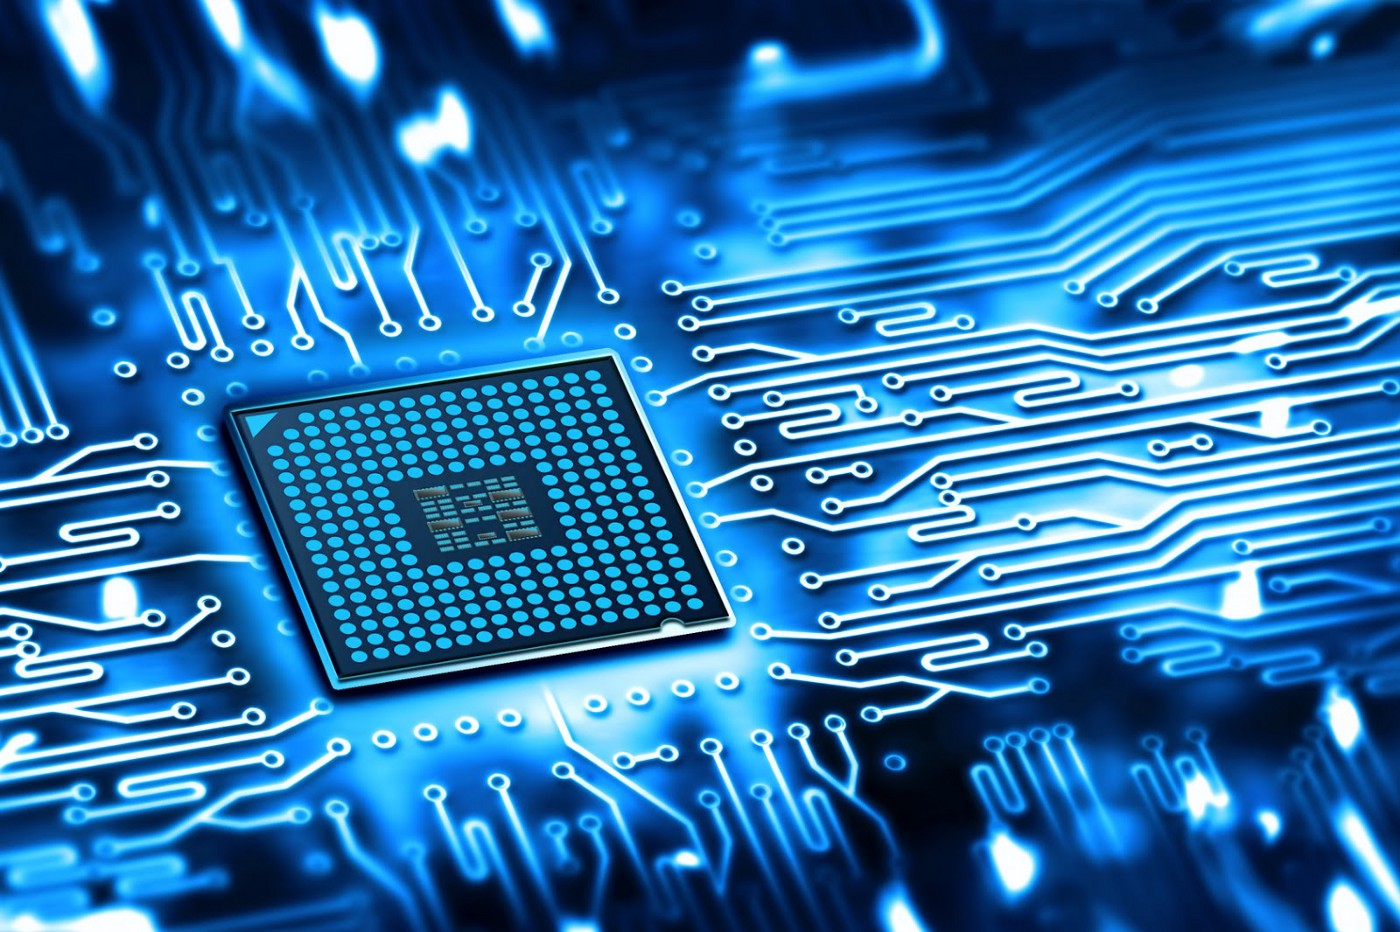
\includegraphics[width=0.6\textwidth]{imgs/circuit}
\end{frame}
\begin{frame}
    \frametitle{What are we going to be talking about?}
    \centering
    \LARGE
    Digital circuits!

    \vspace{1em}
    \normalsize

    \scalebox{2}{\tikzfig{circuits/examples/sr-latch/real-circuit}}
\end{frame}
\begin{frame}
    \frametitle{What are we going to be talking about?}

    \centering
    \Large
    We want a \alert{compositional} theory of digital circuits.

    \vspace{1em}

    \normalsize

    \pause
    \dsptikzfig{strings/category/f}[box=F,colour=seq]
    \pause
    \quad
    \dsptikzfig{strings/category/f}[box=G,colour=seq]
    \pause
    \quad
    \dsptikzfig{strings/category/f-2-2}[box=H,colour=seq]

    \pause
    \vspace{1em}

    \dsptikzfig{strings/category/composition}[box1=F,box2=G,colour=seq]
    \quad
    \dsptikzfig{strings/monoidal/tensor}[box1=F,box2=G,colour=seq]
    \quad
    \dsptikzfig{strings/traced/trace-rhs}[box=H,colour=seq]

    \pause

    \Large
    \vspace{1em}

    Using \alert{string diagrams} removes \\ much of the bureacracy

    \pause

    \normalsize

    (also they look pretty)

\end{frame}

\begin{frame}
    \frametitle{The story so far}

    \centering
    \LARGE

    How did we get here?

    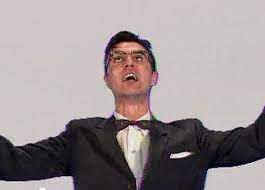
\includegraphics[width=0.5\textwidth]{imgs/byrne}

\end{frame}

\begin{frame}
    \frametitle{The story so far}

    \pause
    \centering

    \scalebox{8}{\textbf{2003}}

\end{frame}

\begin{frame}
    \frametitle{The story so far}

    \centering
    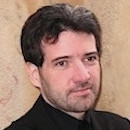
\includegraphics[width=0.3\textwidth]{imgs/lafont}

    \LARGE
    \textbf{Yves Lafont}

    \normalsize
    \emph{`Towards an algebraic theory of Boolean circuits'}

\end{frame}

\begin{frame}
    \frametitle{The story so far}

    \centering

    \scalebox{8}{\textbf{2016}}

\end{frame}

\begin{frame}
    \frametitle{The story so far}

    \centering

    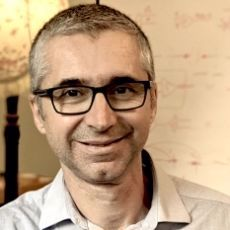
\includegraphics[width=0.25\textwidth]{imgs/ghica}
    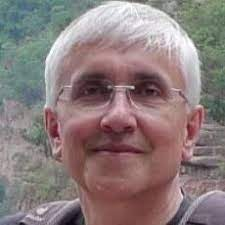
\includegraphics[width=0.25\textwidth]{imgs/achim}
    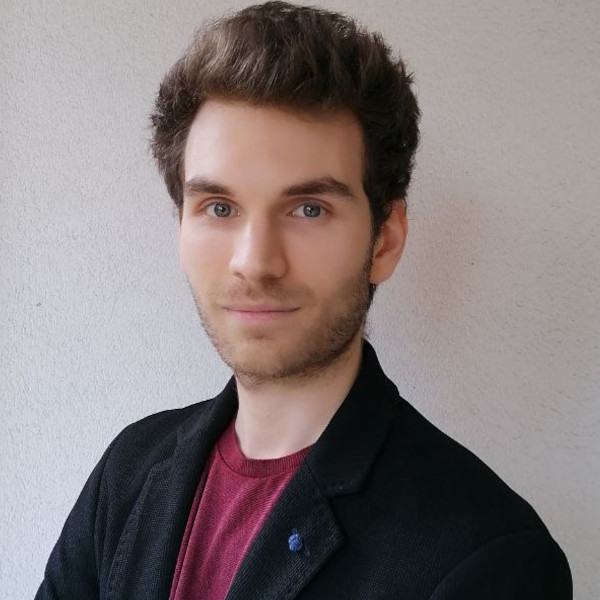
\includegraphics[width=0.25\textwidth]{imgs/lopez}

    \LARGE
    \textbf{Dan Ghica, Achim Jung, Aliaume Lopez}

    \normalsize
    \emph{`Diagrammatic semantics for digital circuits'}


\end{frame}

\begin{frame}
    \frametitle{The story so far}
    \vspace{0.5em}

    \centering

    \pause

    \begin{minipage}{0.49\textwidth}
        \centering
        \only<2>{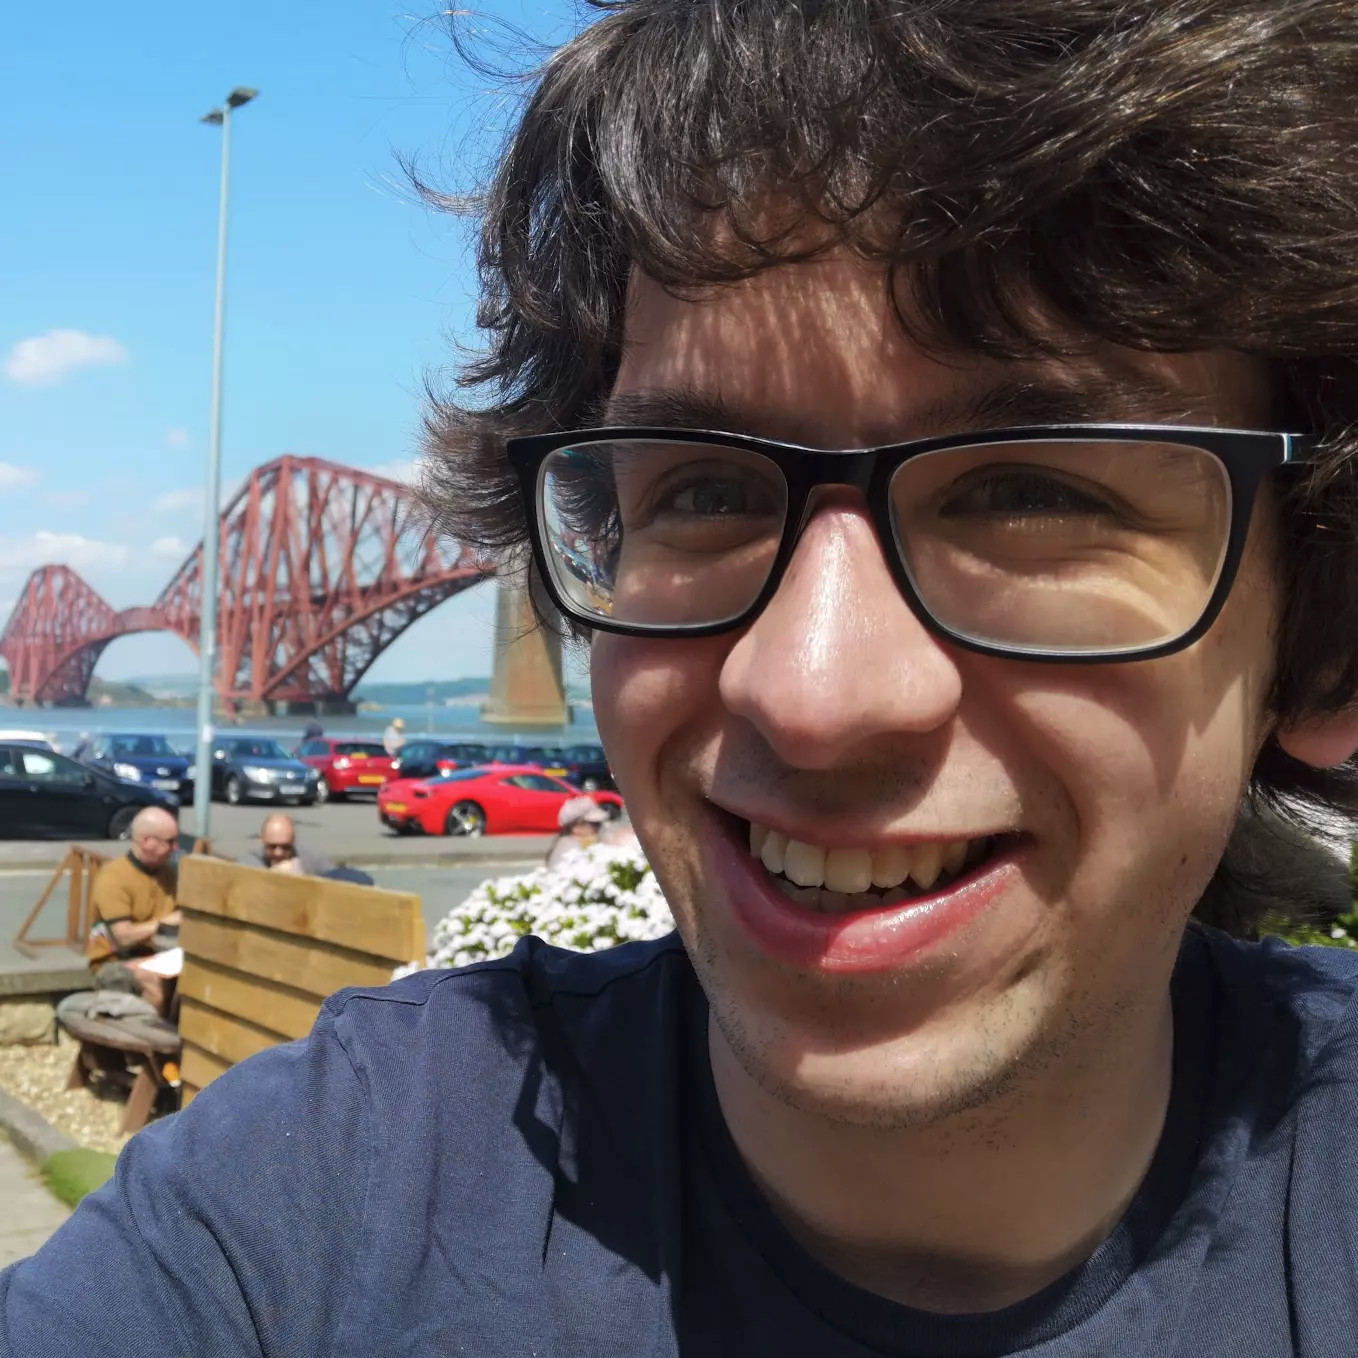
\includegraphics[width=0.5\textwidth]{imgs/kaye}}%
        \only<3->{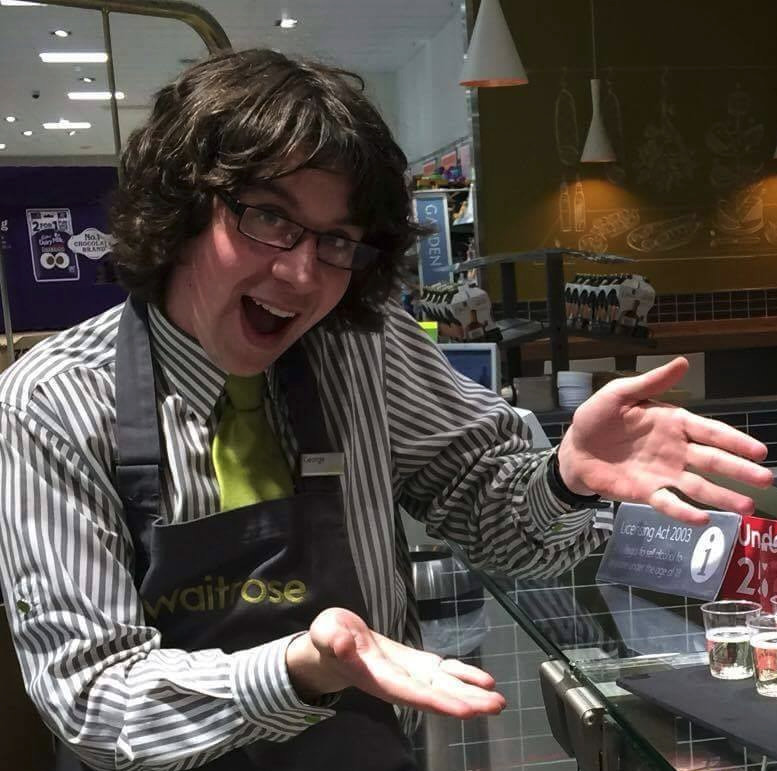
\includegraphics[width=0.5\textwidth]{imgs/kaye-waitrose}}%

        \only<1->{\visible<6->{\emph{`Wow, this guy seems pretty groovy'}}}
    \end{minipage}
    \begin{minipage}{0.49\textwidth}
        \centering
        \only<2-4>{\visible<4>{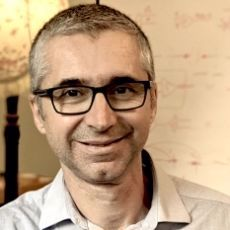
\includegraphics[width=0.5\textwidth]{imgs/ghica}}}%
        \only<5->{
\includegraphics[width=0.5\textwidth]{imgs/ghica-ocaml}}%

        \only<2->{\visible<7>{\emph{*OCaml noises*}}}
    \end{minipage}
\end{frame}

\begin{frame}
    \frametitle{The story so far}

    \centering

    \scalebox{8}{\textbf{2019}}

\end{frame}

\begin{frame}
    \frametitle{The story so far}

    \centering

    \begin{minipage}{0.49\textwidth}
        \centering
        \only<1>{
\includegraphics[width=0.5\textwidth]{imgs/kaye-grad}}%
        \only<2->{
\includegraphics[width=0.5\textwidth]{imgs/kaye-phd}}%

        \visible<5->{\emph{`No'}}

        \visible<7->{\emph{`Okay'}}
    \end{minipage}
    \begin{minipage}{0.49\textwidth}
        \centering
        \visible<3->{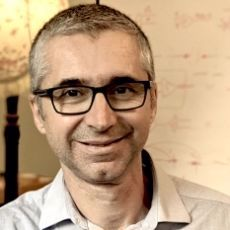
\includegraphics[width=0.5\textwidth]{imgs/ghica}}

        \visible<4->{\emph{`Do you know category theory'}}

        \visible<6->{\emph{`Do you want to do circuits stuff'}}
    \end{minipage}
\end{frame}

\begin{frame}
    \frametitle{The story so far}

    \centering

    \scalebox{8}{\textbf{2021}}

\end{frame}

\begin{frame}
    \frametitle{The story so far}

    \centering

    \vspace{1em}

    \(
        \visible<2->{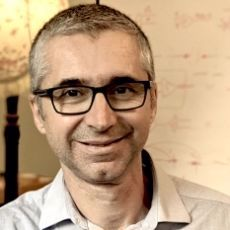
\includegraphics[width=0.2\textwidth]{imgs/ghica}}
        \visible<3->{\raisebox{3em}{ \(+\) }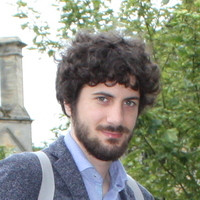
\includegraphics[width=0.2\textwidth]{imgs/zanasi}}
        \visible<4->{\raisebox{3em}{ \(=\) } 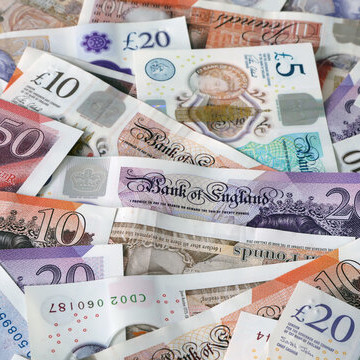
\includegraphics[width=0.2\textwidth]{imgs/money}}
    \)

    \vspace{1em}

    \(
        \visible<5->{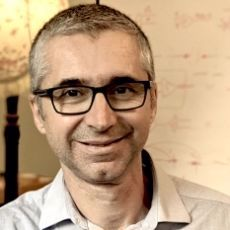
\includegraphics[width=0.2\textwidth]{imgs/ghica}}
        \visible<6->{\raisebox{3em}{ \(+\) }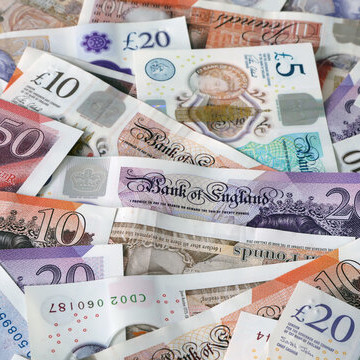
\includegraphics[width=0.2\textwidth]{imgs/money}}
        \visible<7->{\raisebox{3em}{ \(=\) } 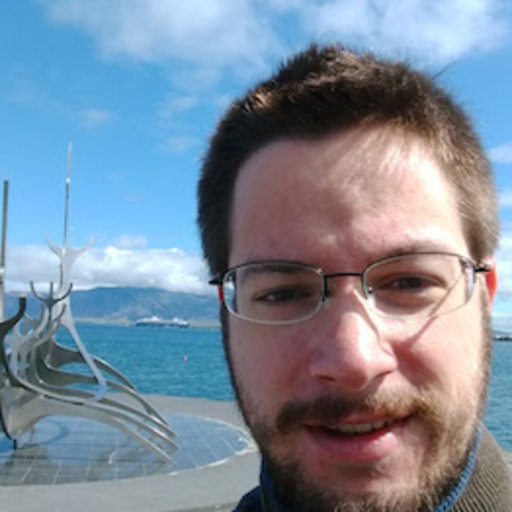
\includegraphics[width=0.2\textwidth]{imgs/sprunger}}
    \)


\end{frame}

\begin{frame}
    \frametitle{The story so far}

    \centering

    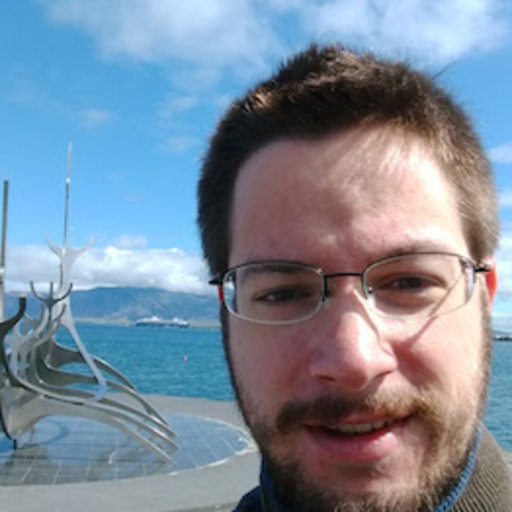
\includegraphics[width=0.25\textwidth]{imgs/sprunger}

    \LARGE
    \textbf{David Sprunger}

    \pause
    \normalsize
    (now at Indiana State University)

\end{frame}

\begin{frame}
    \frametitle{Let's get dangerous}

    \centering

    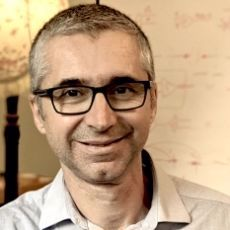
\includegraphics[width=0.25\textwidth]{imgs/ghica}
    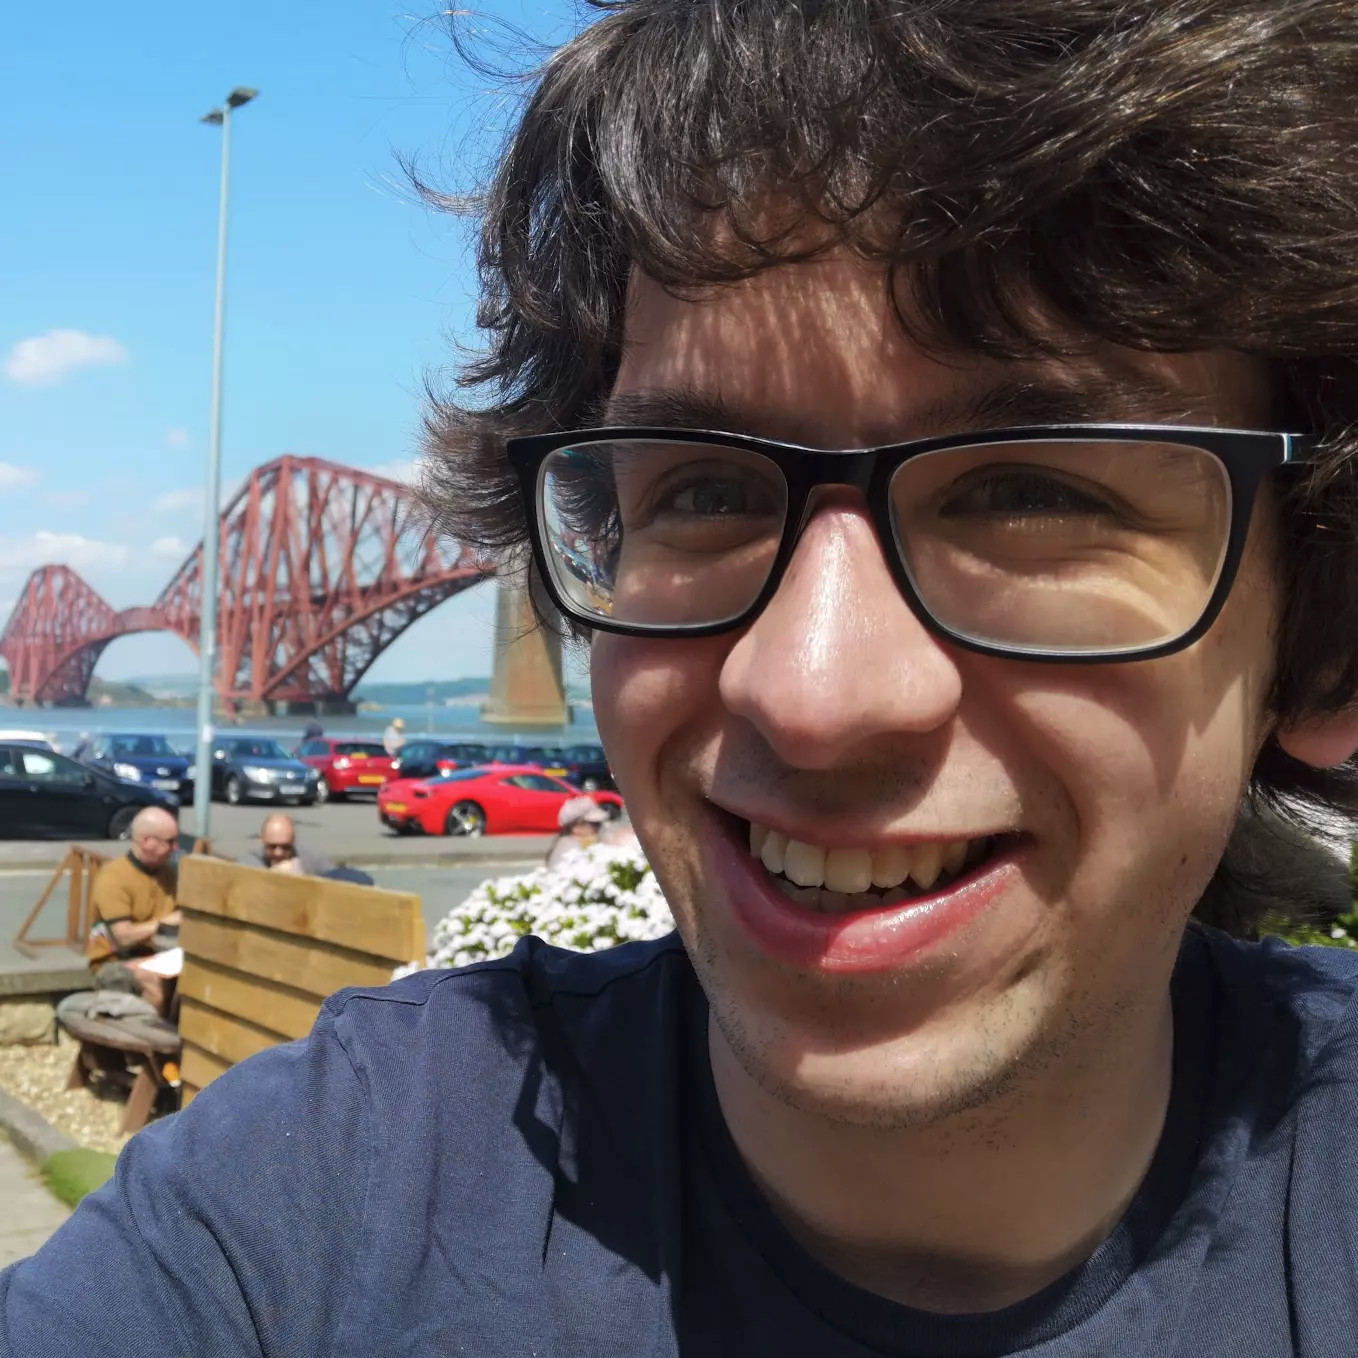
\includegraphics[width=0.25\textwidth]{imgs/kaye}
    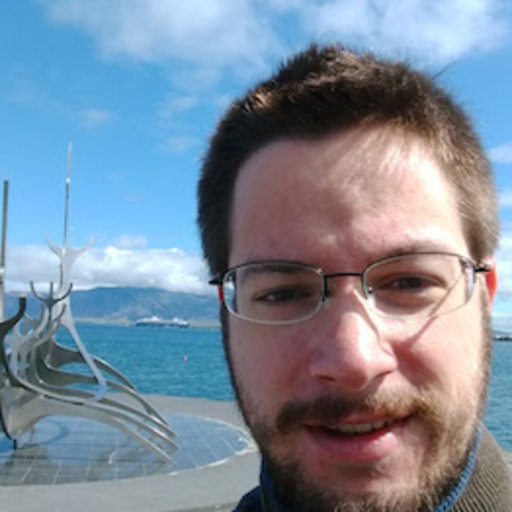
\includegraphics[width=0.25\textwidth]{imgs/sprunger}

\end{frame}
    \section{Syntax}

\begin{frame}
    \frametitle{Combinational circuit components}
    \renewcommand{\arraystretch}{1.25}
    \vspace{1em}
    \pause
    \begin{minipage}{0.33\textwidth}
        \centering
        \alert{gates}
        \renewcommand{\arraystretch}{2}

        \vspace{1em}

        \begin{tabular}{rl}
            \dsptikzfig{circuits/components/gates/and} &
            AND gate \\
            \dsptikzfig{circuits/components/gates/or} &
            OR gate \\
            \dsptikzfig{circuits/components/gates/not} &
            NOT gate \\
        \end{tabular}
    \end{minipage}
    \pause
    \begin{minipage}{0.32\textwidth}
        \centering
        \alert{(co)monoid structure}

        \vspace{1em}

        \renewcommand{\arraystretch}{1.75}
        \pause
        \begin{tabular}{cl}
            \hspace{0.175cm}
            \dsptikzfig{strings/structure/monoid/init}[colour=comb] &
            disconnected \\
            \pause
            \dsptikzfig{strings/structure/comonoid/copy}[colour=comb] &
            fork \\
            \pause
            \dsptikzfig{strings/structure/monoid/merge}[colour=comb] &
            join \\
            \pause
            \dsptikzfig{strings/structure/comonoid/discard}[colour=comb]
            \hspace{0.175cm} &
            stub \\
        \end{tabular}
    \end{minipage}
    \pause
    \begin{minipage}{0.32\textwidth}
        \centering
        \alert{categorical structure}

        \vspace{1em}

        \renewcommand{\arraystretch}{1.75}
        \begin{tabular}{cl}
            \pause
            \dsptikzfig{strings/category/identity}[colour=comb] &
            identity \\
            \pause
            \dsptikzfig{strings/symmetric/symmetry}[colour=comb] &
            symmetry \\
        \end{tabular}
    \end{minipage}


    \vspace{0.5em}

    \pause
    \begin{center}
        \alert{Light} circuits \(
            \dsptikzfig{strings/category/f}[box=F,colour=comb]
        \) only contain gates and structure.
    \end{center}
\end{frame}
\begin{frame}
    \frametitle{Sequential circuit components}

    \renewcommand{\arraystretch}{1.75}

    \pause

    \begin{minipage}{0.3\textwidth}
        \centering
        \alert{Values}

        \pause

        \begin{tabular}{rl}
            \dsptikzfig{circuits/components/values/vs}[val=\belnapfalse] &
            false \\
            \dsptikzfig{circuits/components/values/vs}[val=\belnaptrue] &
            true \\
            \pause
            \dsptikzfig{circuits/components/values/vs}[val=\belnapboth] &
            short circuit
        \end{tabular}

    \end{minipage}
    \pause
    \begin{minipage}{0.3\textwidth}
        \centering
        \alert{Delay}

        \[
            \dsptikzfig{circuits/components/waveforms/delay}
        \]
    \end{minipage}
    \pause
    \begin{minipage}{0.3\textwidth}
        \centering
        \alert{Feedback}

        \[
            \dsptikzfig{strings/category/f-2-2}[box=F,colour=seq]
            \,\,\Rightarrow\,\,
            \dsptikzfig{strings/traced/trace-rhs}[box=F,colour=seq]
        \]
    \end{minipage}

    \vspace{1em}

    \pause

    \begin{center}
        \alert{Dark} circuits \(
            \dsptikzfig{strings/category/f}[box=F,colour=seq]
        \) may contain delay or feedback.
    \end{center}
\end{frame}
\begin{frame}
    \frametitle{Building circuits}

    \centering
    \LARGE
    Circuits are morphisms in a
    \alert{freely generated symmetric traced monoidal category} (STMC).

    \vspace{1em}

    \pause
    \dsptikzfig{strings/category/composition}[box1=F,box2=G,colour=seq]
    \pause
    \quad
    \dsptikzfig{strings/monoidal/tensor}[box1=F,box2=G,colour=seq]
    \pause
    \quad
    \dsptikzfig{strings/traced/trace-rhs}[box=F,colour=seq]

\end{frame}
\begin{frame}
    \frametitle{Need an example?}

    \centering

    \pause

    \tikzfig{circuits/examples/sr-latch/real-circuit}

    \vspace{1em}
    \pause

    \tikzfig{circuits/examples/sr-latch/circuit}


\end{frame}
    \section{Denotational semantics}

\begin{frame}
    \frametitle{We need some meaning}

    \centering

    \huge
    \textbf{What is the meaning?}

\end{frame}

\begin{frame}
    \frametitle{We need some meaning}

    \centering
    \scalebox{4}{\textbf{Denotational}}

    \scalebox{4}{\textbf{semantics}}

\end{frame}

\begin{frame}
    \frametitle{}

    \pause
    Values are interpreted in a \alert{lattice}:

    \pause
    \begin{minipage}{0.49\textwidth}
        \[
            \scalebox{1.5}{\tikzfig{circuits/a4}}
        \]
    \end{minipage}
    \pause
    \begin{minipage}{0.49\textwidth}
        \begin{align*}
            \dsptikzfig{strings/structure/monoid/init}[colour=comb]
            \,&\mapsto\, \bot \\
            \dsptikzfig{circuits/components/values/vs}[val=\belnapfalse]
            \,&\mapsto\, \belnapfalse \\
            \dsptikzfig{circuits/components/values/vs}[val=\belnaptrue]
            \,&\mapsto\, \belnaptrue \\
            \dsptikzfig{circuits/components/values/vs}[val=\top]
            \,&\mapsto\, \top
        \end{align*}
    \end{minipage}
\end{frame}
\begin{frame}
    \frametitle{Let's make everything a function}

    \pause
    \setlength{\tabcolsep}{1.5em}
    \renewcommand{\arraystretch}{2}

    \begin{center}
        \begin{tabular}{lrl}
            \dsptikzfig{circuits/components/gates/gate}[gate=g]
            &
            \alert{monotone functions}
            &
            \(\morph{\overline{g}}{\valuetuple{m}}{\values}\)
            \\
            \pause
            \hspace{0.175cm}
            \dsptikzfig{strings/structure/monoid/init}[colour=comb]
            &
            \alert{initialise}
            &
            \(() \mapsto (\bot)\)
            \\
            \pause
            \dsptikzfig{strings/structure/comonoid/copy}[colour=comb]
            &
            \alert{copy}
            &
            \(x \mapsto (x, x)\)
            \\
            \pause
            \dsptikzfig{strings/structure/monoid/merge}[colour=comb]
            &
            \alert{join in the lattice}
            &
            \((x, y) \mapsto x \ljoin y\)
            \\
            \pause
            \dsptikzfig{strings/structure/comonoid/discard}[colour=comb]
            &
            \alert{discard}
            &
            \(x \mapsto ()\)
        \end{tabular}
        \pause

        \vspace{0.5em}

        Feedback is interpreted as the \alert{least fixed point}.
    \end{center}
\end{frame}
\begin{frame}
        \frametitle{Functions are not enough}

        \centering
        \LARGE
        How do we model \alert{delay}?

        \pause
        \alert{Streams!}
\end{frame}
\begin{frame}
    \frametitle{Streams}

    A \alert{stream} \(\stream{\values}\) is an infinite sequence of values.
    \[
        v_0
        \streamcons
        v_1
        \streamcons
        v_2
        \streamcons
        v_3
        \streamcons
        v_4
        \streamcons
        v_5
        \streamcons
        v_6
        \streamcons
        v_7
        \streamcons
        \cdots
    \]

    \pause
    A \alert{stream function} \(\stream{\values} \to \stream{\values}\) consumes and
    produces streams.
    \[
        f(
            v_0
            \streamcons
            v_1
            \streamcons
            v_2
            \streamcons
            v_3
            \streamcons
            v_4
            \streamcons
            \cdots
        ) =
        w_0
        \streamcons
        w_1
        \streamcons
        w_2
        \streamcons
        w_3
        \streamcons
        w_4
        \streamcons
        \cdots
    \]
\end{frame}
\begin{frame}
    \frametitle{Interpreting the sequential components}

    \LARGE

    \pause
    \[
        \dsptikzfig{circuits/components/values/vs}[val=v]()
        :=
        v \streamcons \bot \streamcons \bot \streamcons \bot \streamcons \cdots
    \]

    \pause
    \vspace{0.5em}

    \[
        \normalsize
        \dsptikzfig{circuits/components/waveforms/delay}
        \LARGE(
            v_0 \streamcons v_1 \streamcons v_2 \streamcons \cdots
        )
        :=
        \bot \streamcons v_0 \streamcons v_1 \streamcons v_2 \streamcons \cdots
    \]
\end{frame}
\begin{frame}{Maybe there are too many streams}

    \centering
    \LARGE
    Does every circuit correspond to a stream function \(
        \valuetuplestream{m} \to \valuetuplestream{n}
    \)?

    \Huge
    \pause
    No.

    \scriptsize
    \pause
    (but this is to be expected!)
\end{frame}
\begin{frame}
    \frametitle{Restricting the stream functions}

    \pause
    \Large
    Circuits are \alert{causal}.

    \pause

    \normalsize
    They can only depend \alert{what they've seen so far}.

    \pause

    \Large
    Circuits are \alert{monotone}.

    \pause

    \normalsize
    They are constructed from \alert{monotone functions}.

    \pause

    Is that all?
    \pause
    \alert{Not quite...}
    \pause
    (but we'll get there)


\end{frame}
\begin{frame}
    \frametitle{Some operations on stream functions}

    Given a causal stream function \(
        \morph{f}{\valuetuplestream{m}}{\valuetuplestream{n}}
    \) and an element \(a \in \valuetuple{m}\)...

    \pause

    \Large
    \alert{initial output} \quad
    \(\mealyoutput{f}{a} \in \valuetuple{n}\)

    \pause

    \normalsize
    `the first thing \(f\) produces given \(a\)'

    \pause

    \Large
    \alert{stream derivative} \quad
    \(\mealytransition{f}{a} \in \valuetuplestream{m} \to \valuetuplestream{n}\)

    \pause

    \normalsize
    `how \(f\) behaves after seeing \(a\) first'

    \vspace{1em}

    \pause
    Hold on, these look familiar...

\end{frame}
\begin{frame}
    \frametitle{An old friend}

    \Large

    \begin{center}
        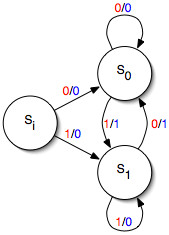
\includegraphics[scale=0.5]{imgs/mealy-machine}

        Mealy machines!

        \pause

        \normalsize
        Stream functions are the \emph{states} in a Mealy machine.
    \end{center}

\end{frame}
\begin{frame}
    \frametitle{Circuits have finitely many behaviours}

    Circuits have a finite number of components.

    \pause

    So there are finite number of states in the Mealy machine.

    \pause

    So the outputs of streams given some input must be \alert{periodic}.

    \pause

    (There are finitely many \alert{stream derivatives}).
\end{frame}
\begin{frame}
    \frametitle{These are the streams we're looking for}

    \begin{theorem}
        A stream function is the interpretation of a sequential circuit
        if and only if it is \textbf{causal}, \textbf{monotone} and has
        \textbf{finitely many stream derivatives}.
    \end{theorem}
\end{frame}
\begin{frame}
    \frametitle{The correspondence}

    \centering
    \Large

    \begin{tikzcd}[ampersand replacement=\&,row sep=large]
        \&
        \text{Circuits}
        \arrow[visible on=<2->]{dl}
        \arrow[visible on=<3->]{dr}
        \&
        \\
        \text{Stream functions}
        \arrow[visible on=<5->,bend left]{ur}
        \arrow[visible on=<4->]{rr}
        \&
        \&
        \text{Mealy machines}
        \arrow[visible on=<5->,bend right]{ul}
        \arrow[visible on=<4->,bend left]{ll}
    \end{tikzcd}
\end{frame}
    % !TeX root = ../main-presentation.tex
\section{Operational semantics}

\begin{frame}
    \frametitle{Doing something useful}

    \centering

    \LARGE
    Suppose we have two circuits \\
    with the same denotation
    \normalsize

    \vspace{2em}

    \(
        \llbracket\dsptikzfig{strings/category/f}[box=F,colour=seq]\rrbracket
        =
        \llbracket\dsptikzfig{strings/category/f}[box=G,colour=seq]\rrbracket
    \)

    \vspace{2em}

    \LARGE
    \await
    What does this tell us about the \\
    \alert{structure} of these circuits?

\end{frame}
\begin{frame}
    \frametitle{Reducing it down}

    \await

    \centering
    \scalebox{4}{\textbf{Operational}}

    \scalebox{4}{\textbf{semantics}}

\end{frame}
\begin{frame}
    \frametitle{Reducing it down}

    \centering
    \LARGE

    We want to find a set of \\ \alert{reductions} for digital circuits


    \await
    We want to reduce circuits to their outputs \alert{syntactically}
    in a \alert{step-by-step} manner

\end{frame}
\begin{frame}
    \frametitle{Going global}

    \centering

    \dsptikzfig{strings/category/f}[box=F,colour=seq]
    \await
    \Large=\normalsize
    \dsptikzfig{circuits/productivity/trace-delay}[core=\hat{F},state=\listvar{v}]

    \vspace{1em}
    \Large
    by moving boxes and wires around
\end{frame}

\begin{frame}
    \frametitle{Going global}

    \centering
    \Large

    \await

    \normalsize
    \begin{gather*}
        \dsptikzfig{circuits/components/waveforms/register}
        \coloneqq
        \dsptikzfig{circuits/components/waveforms/register-shorthand}
        \qquad
        \Large
        \text{\alert{`Register'}}
    \end{gather*}

    \vspace{1em}

    \await

    \dsptikzfig{circuits/productivity/trace-delay}[core=F,state=\listvar{v}]
    \Large\(\reduction\)\normalsize
    \dsptikzfig{circuits/productivity/mealy-rule}

    \await

    \dsptikzfig{strings/category/f}[box=F,colour=seq]
    \Large\(\reductions\)\normalsize
    \dsptikzfig{circuits/productivity/pre-mealy-form}[core=\hat{F},state=\listvar{s}]

\end{frame}
\begin{frame}
    \frametitle{The sticking point}

    \centering

    What are we going to do about the non-delay-guarded trace?

    \await

    In industry, feedback is usually \alert{delay-guarded}.

    \await

    But this rules out some \alert{clever} circuits!

    \normalsize

    \vspace{1em}

    \scalebox{0.75}{
        \dsptikzfig{circuits/examples/cyclic-combinational/circuit-scirc}
        \(\Rightarrow\)
        \dsptikzfig{circuits/examples/cyclic-combinational/reduced-true}
    }

    \await

    \vspace{1em}

    \scriptsize
    (And also it would be cheating)

\end{frame}
\begin{frame}
    \frametitle{Getting rid of non-delay-guarded feedback}

    \centering
    \LARGE

    \(\values\) is a \alert{finite} lattice...\

    \await
    The functions are monotone...

    \await
    We can compute the \alert{least fixed point} \\ in finite iterations!

\end{frame}
\begin{frame}
    \frametitle{Getting rid of non-delay-guarded feedback}

    \centering
    \[
        \dsptikzfig{circuits/instant-feedback/f0-box}
        \coloneqq
        \dsptikzfig{circuits/instant-feedback/f0-definition}
        \await
        \qquad
        \dsptikzfig{circuits/instant-feedback/fkp1-box}
        \coloneqq
        \dsptikzfig{circuits/instant-feedback/fkp1-definition}
    \]
    \await
    \[
        \dsptikzfig{circuits/instant-feedback/equation-lhs}[box=F,trace=x]
        \quad
        \reduction
        \quad
        \dsptikzfig{circuits/instant-feedback/fixpoint-concrete}
    \]

\end{frame}
\begin{frame}
    \frametitle{Getting rid of non-delay-guarded feedback}


    \[
        \dsptikzfig{circuits/instant-feedback/trand}
        \quad
        \await
        \reduction
        \quad
        \dsptikzfig{circuits/instant-feedback/trand-instfb}
    \]


\end{frame}
\begin{frame}
    \frametitle{Here's Mealy}

    \centering
    \Large
    For \alert{any} circuit
    \normalsize

    \[
        \dsptikzfig{strings/category/f}[box=F,colour=seq]
        \quad
        \reductions
        \quad
        \dsptikzfig{circuits/productivity/mealy-form}[core=\tilde{F},state=\overline{s}]
    \]

\end{frame}
\begin{frame}
    \frametitle{What is the goal}

    \centering

    \await
    \Large
    We want to compute the \alert{outputs} of circuits given some \alert{inputs}
    \normalsize

    \begin{gather*}
        \dsptikzfig{circuits/productivity/productive-goal-lhs}[box=F]
        \reductions
        \dsptikzfig{circuits/productivity/productive-goal-rhs}[box=G]
    \end{gather*}

    \await

    \vspace{1em}

    \Large

    How does a circuit \alert{process} a value?

\end{frame}
\begin{frame}
    \frametitle{Reducing values}

    \begin{gather*}
        \dsptikzfig{circuits/axioms/gate-lhs}
        \reduction
        \dsptikzfig{circuits/axioms/gate-rhs}
        \qquad
        \dsptikzfig{circuits/axioms/fork-lhs}
        \reduction
        \dsptikzfig{circuits/axioms/fork-rhs}
        \\[0.5em]
        \dsptikzfig{circuits/axioms/join-lhs}
        \reduction
        \dsptikzfig{circuits/axioms/join-rhs}
        \qquad
        \dsptikzfig{circuits/axioms/stub-lhs}
        \reduction
        \dsptikzfig{strings/monoidal/empty}
    \end{gather*}

    \await`'
    \vspace{1em}
    \Large

    \begin{lemma}
        For every
        \dsptikzfig{strings/category/f}[box=F,colour=comb]
        there exists
        \dsptikzfig{circuits/components/values/vs}[val=\listvar{w}]
        s.t.
        \dsptikzfig{circuits/components/circuits/f-applied}[box=F,colour=comb]
        \(\reduction\)
        \dsptikzfig{circuits/components/values/vs}[val=\listvar{w}].
    \end{lemma}

\end{frame}


\begin{frame}
    \frametitle{Catching the jet stream}

    \Large

    What about \alert{delays}?

    \normalsize

    \begin{gather*}
        \visible<\iftoggle{static}{1}{2-}>{\dsptikzfig{circuits/axioms/generalised-streaming-lhs}[box=F]}
        \visible<\iftoggle{static}{1}{3-}>{\coloneqq}
        \visible<\iftoggle{static}{1}{3-}>{\dsptikzfig{circuits/axioms/generalised-streaming-lhs-verbose}[box=F]}
        \visible<\iftoggle{static}{1}{4-}>{\reduction}
        \visible<\iftoggle{static}{1}{4-}>{\dsptikzfig{circuits/axioms/generalised-streaming-rhs}[box=F]}
        \qquad
        \visible<\iftoggle{static}{1}{5-}>{\text{\alert{'Streaming'}}}
    \end{gather*}
\end{frame}

\begin{frame}
    \frametitle{Catching the jet stream}

    \vspace{-2em}

    \begin{gather*}
        \visible<\iftoggle{static}{1}{2-}>{\dsptikzfig{circuits/productivity/productive-goal-lhs}[box=F]}
        \visible<\iftoggle{static}{1}{3-}>{\reduction}
        \visible<\iftoggle{static}{1}{3-}>{\dsptikzfig{circuits/productivity/mealy-form-applied}[core=\hat{F}]}
        \visible<\iftoggle{static}{1}{4-}>{\reduction}
        \visible<\iftoggle{static}{1}{4-}>{\dsptikzfig{circuits/productivity/mealy-form-streamed}[core=\hat{F}]}
        \\[0.5em]
        \visible<\iftoggle{static}{1}{5-}>{\reduction}
        \visible<\iftoggle{static}{1}{5-}>{\dsptikzfig{circuits/productivity/mealy-form-instant}[core=\hat{F}]}
        \visible<\iftoggle{static}{1}{6-}>{\reduction}
        \visible<\iftoggle{static}{1}{6-}>{\dsptikzfig{circuits/productivity/mealy-form-instant-registers}[core=\hat{F}]}
        \\[0.5em]
        \visible<\iftoggle{static}{1}{7-}>{\reduction}
        \visible<\iftoggle{static}{1}{7-}>{\dsptikzfig{circuits/productivity/mealy-form-produced}[core=\hat{F}]}
        \visible<\iftoggle{static}{1}{8-}>{\coloneqq}
        \visible<\iftoggle{static}{1}{8-}>{\dsptikzfig{circuits/productivity/productive-goal-rhs}[box=G]}
    \end{gather*}
\end{frame}

\begin{frame}
    \frametitle{Observe this}

    \centering
    \LARGE

    When are two circuits \alert{observationally equivalent}?

    \await

    Circuits have \alert{finitely many states}...

    \vspace{1em}

    \await
    \Large
    \begin{definition}
        Two circuits with at most \(c\) delay components are observationally
        equivalent if the reduction procedure creates the same outputs for all
        inputs of length \(|\values|^c+1\).
    \end{definition}

\end{frame}

\begin{frame}
    \frametitle{Observe this}

    \centering
    \Large

    \begin{theorem}
        Two circuits are observationally equivalent if and only if they are
        denotationally equivalent.
    \end{theorem}

    \await

    Sound and complete \alert{operational semantics}


\end{frame}
    % !TeX root = ../main-presentation.tex
\section{From diagrams to graphs}

\begin{frame}
    \frametitle{Making it combinatorial}

    \centering

    \pause

    \dsptikzfig{circuits/productivity/mealy-form}
    \Large
    \pause
    \(\Rightarrow\)
    \raisebox{-2em}{
\includegraphics[scale=0.5]{crash}}

    \pause

    \vspace{1.5em}

    It is \alert{hard} for computers to work with string diagrams...

    \pause

    ...but computers \alert{love} graphs!

\end{frame}

\begin{frame}
    \frametitle{A hyper kind of graph}

    \centering

    \dsptikzfig{graphs/example-trace-cospan}

    \vspace{1em}

    \pause
    \Large

    There are correspondences between \alert{certain classes of hypergraphs} and
    \alert{circuit string diagrams}.

    \pause
    \normalsize
    \vspace{1em}

    \dsptikzfig{graphs/example-trace-term}

\end{frame}

\begin{frame}
    \frametitle{Using the correspondence}

    \centering
    \Large

    \begin{tikzcd}[ampersand replacement=\&]
        |[visible on=<1->]|\text{Circuit string diagram}
        \arrow[visible on=<2->]{r}
        \arrow[visible on=<5->, equals]{d}
        \&
        |[visible on=<2->]|\text{Hypergraph representation}
        \arrow[visible on=<3->]{d}{\text{\alert{Graph rewrite}}}
        \\
        |[visible on=<4->]|\text{New circuit string diagram}
        \&
        |[visible on=<3->]|\text{Rewritten hypergraph}
        \arrow[visible on=<4->]{l}
    \end{tikzcd}

\end{frame}

\begin{frame}
    \frametitle{Implementing it all}

    \centering
    \Large

    The rewriting framework has been \emph{implemented} in a
    \alert{hardware description language}.

    \begin{center}
        
\includegraphics[width=0.2\textwidth]{huawei}
    \end{center}

    \pause

    \small
    (the language is still in development)

    \pause

    \scriptsize
    (so I've been warned not to accidentally announce anything)

\end{frame}

\begin{frame}
    \frametitle{I can still show you something}

    Create a circuit...

    \svg{0}{0.5}{acc}

\end{frame}
\begin{frame}
    \frametitle{I can still show you something}

    The evaluator converts it into \alert{Mealy form}...

    \svg{0}{0.25}{eval-0}

\end{frame}
\begin{frame}
    \frametitle{I can still show you something}

    ...and then evaluates an input.

    \svg{0}{0.2}{after-1}
    \raisebox{5em}{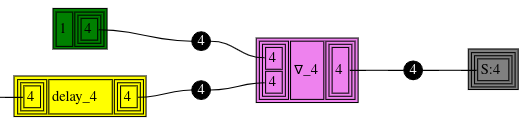
\includegraphics[scale=1.5]{output-1}}

\end{frame}

    \begin{frame}
        \frametitle{Conclusion}

        We have developed a \alert{compositional framework} for digital circuits

        \pause

        We have an \alert{operational semantics} for digital circuits

        \pause

        We can model this using \alert{graph rewrites} on \alert{hypergraphs}

        \pause

        This has been \alert{implemented} in a hardware description language

    \end{frame}
\end{document}